\documentclass{article}

%=====================================================================
%============================= packages ==============================

%\usepackage{geometry}
\usepackage{amsmath}
\usepackage{amssymb}
\usepackage{stmaryrd}
\usepackage{fancyhdr}
\usepackage{natbib}
\usepackage[normalem]{ulem}
\usepackage{examples-slim}
\usepackage{xcolor}
\usepackage{graphicx}
\usepackage{float}
\usepackage{multirow}
\usepackage{booktabs}
\usepackage{colortbl}
\usepackage{caption}
\usepackage{subcaption}
\definecolor{black}{rgb}{0,0,0}
\usepackage[colorlinks, linkcolor=black, urlcolor=black, citecolor=black]{hyperref}

\bibpunct[; ]{(}{)}{;}{a}{}{,}  % natbib citation style

%=====================================================================
%========================= cross-references ==========================

% Flexible sec/fig/tbl/def cross-refs.
\newcommand{\Secref}[1]{Section~\ref{#1}}
\newcommand{\secref}[1]{section~\ref{#1}}
\newcommand{\dashsecref}[2]{sections~\ref{#1}--\ref{#2}}

\newcommand{\Defref}[1]{Def.~\ref{#1}}
\newcommand{\defref}[1]{def.~\ref{#1}}
\newcommand{\Defrefc}[2]{\Defref{#1}, clause~\ref{#2}}
\newcommand{\defrefc}[2]{\defref{#1}, clause~\ref{#2}}

\newcommand{\Figref}[1]{Figure~\ref{#1}}
\newcommand{\figref}[1]{figure~\ref{#1}}
\newcommand{\dashfigref}[2]{figures~\ref{#1}--\ref{#2}}
\newcommand{\Tabref}[1]{Table~\ref{#1}}
\newcommand{\tabref}[1]{table~\ref{#1}}

% Examples:
\newcommand{\eg}[1]{(\ref{#1})}
\newcommand{\subeg}[2]{(\ref{#1}\ref{#2})}
\newcommand{\dblsubeg}[3]{(\ref{#1}\ref{#2},~\ref{#3})}
\newcommand{\dashsubeg}[3]{(\ref{#1}\ref{#2}--\ref{#3})}

% In-text citations
\newcommand{\posscitet}[1]{\citeauthor{#1}'s~(\citeyear{#1})}
\newcommand{\sposscitet}[1]{\citeauthor{#1}'~(\citeyear{#1})}
\newcommand{\possciteauthor}[1]{\citeauthor{#1}'s}
\newcommand{\spossciteauthor}[1]{\citeauthor{#1}'}
\newcommand{\pgposscitet}[2]{\citeauthor{#1}'s~(\citeyear{#1}:~#2)}
\newcommand{\secposscitet}[2]{\citeauthor{#1}'s~(\citeyear{#1}:~$\S$#2)}
\newcommand{\pgcitealt}[2]{\citealt{#1}:~#2}
\newcommand{\seccitealt}[2]{\citealt{#1}:~$\S$#2}
\newcommand{\pgcitep}[2]{(\citealt{#1}:~#2)}
\newcommand{\seccitep}[2]{(\citealt{#1}:~$\S$#2)}
\newcommand{\pgcitet}[2]{\citeauthor{#1}~(\citeyear{#1}:~#2)}
\newcommand{\seccitet}[2]{\citeauthor{#1}~(\citeyear{#1}:~$\S$#2)}

%=====================================================================
%============================ text styles ============================

\newcommand{\word}[1]{\emph{#1}}
\newcommand{\tech}[1]{\textbf{#1}}
\definecolor{maroon}{HTML}{990000}
\newcommand{\highlight}[1]{{\color{maroon}#1}}

%=====================================================================
%============================== judgments ============================

\newcommand{\bad}{\sqz{${}^\ast$}}
\newcommand{\freebad}{${}^\ast$}
\newcommand{\marked}{\sqz{${}^\#$}}
\newcommand{\freemarked}{${}^\#$}

%=====================================================================
%=============================== model ===============================


\newcommand{\tuple}[1]{\ensuremath{\left< #1 \right>}}
\newcommand{\set}[1]{\ensuremath{\left\{ #1 \right\}}}
\newcommand{\True}{\texttt{T}}
\newcommand{\False}{\texttt{F}}
\newcommand{\Reals}{\mathbb{R}}
\newcommand{\given}{\mid}
\newcommand{\Indicator}{\mathbb{I}}

\newcommand{\sem}[1]{\ensuremath{\llbracket#1\rrbracket}}
\newcommand{\States}{W}
\newcommand{\state}{w}
\newcommand{\Lex}{\mathcal{L}}
\newcommand{\LexStar}{\Lex^{\ast}}
\newcommand{\LexSet}{\mathbf{L}}
\newcommand{\Messages}{M}
\newcommand{\msg}{m}
\newcommand{\Costs}{C}
\newcommand{\Prior}{P}
\newcommand{\LexPrior}{P_{\LexSet}}

\newcommand{\listenerZero}{l_{0}}
\newcommand{\speakerOne}{s_{1}}
\newcommand{\listenerOne}{l_{1}}
\newcommand{\SpeakerK}[1][k]{S_{#1}}
\newcommand{\ListenerK}[1][k]{L_{#1}}

\newcommand{\nullmsg}{\mathbf{0}}

%=====================================================================
%============================ annotations ============================

\let\oldmarginpar\marginpar
\renewcommand{\marginpar}[1]{\oldmarginpar[\color{red}\raggedright\scriptsize #1]{\color{red}\raggedright\scriptsize #1}}

\newcommand{\textnote}[1]{{\color{red}#1}}

%=====================================================================
%============================== colors ===============================

\definecolor{lightgray}{HTML}{CCCCCC} 

\definecolor{highlightcolor}{HTML}{D95F02}
\definecolor{annotationcolor}{HTML}{777777} 
\definecolor{worldinfocolor}{HTML}{E7298A}
\definecolor{lexcolor}{HTML}{D95F02}
\definecolor{costcolor}{HTML}{A6761D}
\definecolor{defcolor}{HTML}{D95F02}
%\definecolor{hurfordcolor}{HTML}{00CC33}
\definecolor{hurfordcolor}{HTML}{1B9E77}
\newcommand{\hurford}[1]{{\relax\color{hurfordcolor}#1}}
\newcommand{\definitional}[1]{\relax{\color{defcolor}#1}}

\newcommand{\graycell}[1]{{\cellcolor[gray]{.8}#1}}

%=====================================================================
%============================== helpers ==============================

\newcommand{\porq}{p\,\word{or}\,q}
\newcommand{\pandq}{p\,\&\,q}

\newcommand{\disjlexicon}[2]{
  \left[
    \begin{array}[c]{l@{ \ \mapsto \ } l}
      \porq    & \set{#1} \\
      \pandq   & \set{#2} \\
      \nullmsg & \set{w_{1}, w_{2}, w_{3}} \\
    \end{array}
  \right]}

\newcommand{\listenerMatrix}[6]{
  \begin{array}[c]{l *{4}{r}}
    \toprule
    #1 & w_{1} & w_{2} & w_{3} \\
    \midrule
    p        & #2 \\
    q        & #3 \\              
    \pandq   & #4 \\
    \porq    & #5 \\
    \nullmsg & #6 \\
    \bottomrule
  \end{array}}

\newcommand{\speakerMatrix}[4]{
  \begin{array}[c]{r *{5}{r}}
    \toprule
    #1 & p & q & \pandq & \porq & \nullmsg \\
    \midrule
    w_{1} & #2 \\
    w_{2} & #3 \\ 
    w_{3} & #4 \\ 
    \bottomrule
  \end{array}}

\newcommand{\ListenerKMatrix}[4]{
  \begin{array}[c]{l *{3}{r}}
  \toprule
    #1 & w_{1} & w_{2} & w_{3} \\
    \midrule
    \LexStar  & #2 \\
    \Lex_{1}  & #3 \\
    \Lex_{2}  & #4 \\
    \bottomrule
  \end{array}}

\newcommand{\SpeakerKMatrix}[4]{
  \begin{array}[c]{l *{3}{r}}
    \toprule
    \Lex_{#1} & \porq & \pandq & \nullmsg \\
    \midrule
    w_{1}  & #2 \\
    w_{2}  & #3 \\
    w_{3}  & #4 \\
    \bottomrule
  \end{array}}

\newcommand{\smalldisjlex}[3]{
  \setlength{\arraycolsep}{1pt}
  \left[
    \begin{array}[c]{l@{ \ \mapsto \ }r@{, \ } l@{ \ \mapsto \ }r@{, \ } l@{ \ \mapsto \ }r}
      A & \set{#1} &
      B & \set{#2} &
      X & \set{#3}
    \end{array}
  \right]}

\newcommand{\smalldisjlexTargetDef}{\smalldisjlex{\definitional{\mathbf{w_{1}}}}{w_{2}}{\definitional{\mathbf{w_{1}}}}}

\newcommand{\smalldisjlexTargetHuford}{\smalldisjlex{\hurford{\mathbf{w_{1}}}}{w_{2}}{\hurford{\mathbf{w_{2}}}}}

\definecolor{highlightcolor}{HTML}{D95F02}
\definecolor{annotationcolor}{HTML}{777777} 
\definecolor{worldinfocolor}{HTML}{E7298A}
\definecolor{lexcolor}{HTML}{D95F02}
\definecolor{costcolor}{HTML}{A6761D}
\definecolor{defcolor}{HTML}{D95F02}
\definecolor{hurfordcolor}{HTML}{00CC33}
\newcommand{\hurford}[1]{{\relax\color{hurfordcolor}#1}}
\newcommand{\definitional}[1]{\relax{\color{defcolor}#1}}

\definecolor{lightgray}{HTML}{CCCCCC} 
%\renewcommand{\graycell}[1]{\colorbox{lightgray}{#1}}
\newcommand{\whitecell}[1]{\colorbox{white}{#1}}

\newcommand{\lismat}[4]{
  \setlength{\arraycolsep}{1pt}
  \begin{array}[c]{l *{3}{r}}
    \toprule
    #1 & w_{1} & w_{2} & w_{1}{\vee}w_{2} \\
    \midrule
    A & #2\\
    X & #3 \\
    A\,\word{or}\,X & #4 \\
    \bottomrule
  \end{array}}

\newcommand{\spkmat}[4]{
  \setlength{\arraycolsep}{1pt}
  \begin{array}[c]{l *{3}{r}}
    \toprule
    #1 & A & X & A\,\word{or}\,X \\
    \midrule
    w_{1} & #2\\
    w_{2} & #3 \\
    w_{1}{\vee}w_{2} & #4 \\
    \bottomrule      
  \end{array}}                   

\renewcommand{\disjlexicon}[2]{
  \renewcommand{\arraystretch}{1}
  \left[   
    \begin{array}[c]{l@{ \ \mapsto \ } l}
      p   & \set{#1} \\
      q  & \set{#2} \\
    \end{array}
  \right]}

\newcommand{\closurelex}[6][1]{
  \renewcommand{\arraystretch}{1}
  \begin{array}[c]{*{8}{r}}
    \toprule
    &w_{1}&w_{2}&w_{3}&w_{1}{\vee}w_{2}&w_{1}{\vee}w_{3}&w_{2}{\vee}w_{3}&w_{1}{\vee}w_{2}{\vee}w_{3}\\
    \midrule
    p      & #2 \\
    q      & #4 \\
    \pandq & #3 \\
    \porq  & #5 \\
    \nullmsg & #6 \\
    \bottomrule
  \end{array}}


\begin{document}

%%%%%%%%%%%%%%%%%%%%%%%%%%%%%%%%%%%%%%%%%%%%%%%%%%%%%%%%%%%%%%%%%%%%%%

\title{Negotiating lexical uncertainty and expertise with disjunctive utterances}
\author{Roger Levy and Christopher Potts}
\maketitle

%%%%%%%%%%%%%%%%%%%%%%%%%%%%%%%%%%%%%%%%%%%%%%%%%%%%%%%%%%%%%%%%%%%%%%

\section{Communicating in language about language}\label{sec:introduction}

Natural languages are neither fixed across time nor identically
reproduced in all speakers, but rather continually renegotiated during
interactions \citep{Clark97}. Discourse participants accommodate to
each other's usage patterns \citep{Giles:Coupland:Coupland:1991}, form
temporarily lexical pacts to facilitate communication
\citep{Clark:Wilkes-Gibbs:1986,Brennan:Clark:1996}, and instruct each
other about their linguistic views. Some of this communication in
language about language is direct, as with explicit definitions like
\word{`oenophile' means wine lover}, but much of it arrives via
secondary pragmatic inferences, as when \word{X such as Y} conveys
that \word{X} subsumes \word{Y} \citep{Hearst92,SnowEtAl05}.

Disjunction supports what appear to be opposing inferences about
language. On the one hand, \word{X or Y} tends to convey that the
meanings of \word{X} and \word{Y} are presumed to be disjoint
\citep{Hurford:1974}, because the speaker holds such a view of the
lexicon or is worried that the listener might. This pressure to
exclusivize is robust enough to overcome even seemingly non-negotiable
aspects of the lexicon; a medical webpage warns ``If you still have
symptoms or severe blockage in your arteries, you may need angioplasty
or surgery'', sending a clear signal that angioplasty and surgery
are distinct options. Its continuation presupposes just that: 
``Having one of these procedures may save your leg''. The disjunction
might seem to be a needlessly verbose way of conveying the meaning of
the more general disjunct, but the costs could be worth paying in
virtue of the lexical side-effect of exclusivization.

On the other hand, disjunctions like \word{wine lover or oenophile}
can be used to convey that the two disjuncts are roughly synonymous
\citep{Horn89}, thereby providing secondary information that maximally
violates the pressure to exclusivize. This inference is more rarefied
than the exclusivization inference, but it can arise in a broad range
of contexts in which such definitional or identificational information
has social or communicative value. It is striking that the
definitional and exclusivization inferences are supported by a single
lexical item, and the puzzle deepens when we see that the empirical
picture is not a quirk of English, but rather one that we find in a
wide range of typologically and geographically diverse languages.

In this paper, we capture both of these classes of inference within a
single recursive Bayesian model of pragmatic reasoning. The model
finds its conceptual origins in \posscitet{Lewis69} work on signaling
systems and builds on ideas from iterated best response models
\citep{Jaeger:2007,Jaeger:2011,Franke09DISS} and more thoroughly
probabilistic variants of them
\citep{CamererHo:2004,Frank:Goodman:2012}. The crucial feature of our
model is that it lets discourse participants communicate, not just
about the world, but also about the language they are using
\citep{Bergen:Goodman:Levy:2012,bergen-levy-goodman:2014}: the
speaker's intentions in production are characterized in terms of both
world information and linguistic information, and the listener's
pragmatic reasoning is cast as a problem of joint inference about the
speaker's intended meaning and preferred lexicon
\citep{Smith:Goodman:Frank:2013}. We show that, within this model,
both exclusivization and definitional inferences arise naturally from
the expected semantic content of disjunction, depending on contextual
parameters relating to speaker expertise, listener malleability, and
information contained in the common ground. The model thus offers a
genuinely pragmatic account of these inferences as well as
characterizations of their stability and their communicative value.

%%%%%%%%%%%%%%%%%%%%%%%%%%%%%%%%%%%%%%%%%%%%%%%%%%%%%%%%%%%%%%%%%%%%%%

\section{Lexical side-effects from disjunction}\label{sec:data}

This section explores the exclusivization and identificational uses of
disjunction. Our goal is to more precisely characterize what the
inferences are like and to begin to characterize which context steer
speakers and listeners toward one or the other. These findings inform
the modeling we describe in \dashsecref{sec:model}{sec:analysis}.

%=====================================================================

\subsection{Hurfordian perceptions and intentions}\label{sec:data:overlapping}

\posscitet{Hurford:1974} generalization (HG) is a direct statement of
the overall communicative pressure to treat disjuncts as exclusive:
%
\begin{quote}
  ``The joining of two sentences by \word{or} is unacceptable if one
  sentence entails the other; otherwise the use of \word{or} is
  acceptable.'' (p.~410)
\end{quote}
%
The generalization is stated in terms of sentences, but Hurford's
examples, given in \eg{hex} with his original judgments, make it clear
that he intends it to hold for sub-sentential disjuncts as well (he is
likely assuming conjunction reduction):
%
\begin{examples}
\item\label{hex}
  \begin{examples}
  \item Ivan is an American or Russian.
  \item The painting is of a man or a woman.
  \item The value of $x$ is greater than or equal to 6.
  \item\label{ex-bad1}\bad John is an American or Californian.
  \item\label{ex-bad2}\bad The painting is of a man or a bachelor.
  \item\label{ex-bad3}\bad The value of $x$ is greater than or not equal to 6.
  \end{examples}
\end{examples}

\citeauthor{Hurford:1974} uses HG to probe the nature and distribution
of conversational implicatures (see also
\citealt{Gazdar79b,ChierchiaFoxSpector08}), and \citet{Singh:2008}
extends it to cases in which the disjuncts are merely overlapping. We
endorse the guiding insight behind these accounts but reject the
assumption that HG violations reliably lead to, or even correlate
with, unacceptability or ungrammaticality. Disjunctions of apparently
entailing phrases are routine; all of the examples marked as
ungrammatical in \eg{hex} are easy to find in fluent English text on
the Web:
%
\begin{examples}
\item\label{hex-good}
  \begin{examples}
  %\item ``How much does the average american or californian pay every
  %  year toward state taxes?''
  \item ``\ldots and we trust that some of our \highlight{American or
      Californian} friends will tell us something of its growth of
    flower and fruit in its native habitats''
  \item ``It doesn't matter if you ask \highlight{a boy or a man or a
      bachelor or even a husband}, \ldots''
  \item ``the effect was \highlight{greater than, or not equal to,}
    the cause.''
  \end{examples}
\end{examples}

We have collected a large corpus of apparent counterexamples,
available at \url{http://goo.gl/VAGqnB}. Here is a small sample from
that corpus:
%
\begin{examples}
\item\label{ourcorpus} 
  %
  \begin{examples}
    %%%%%%%%%% X < Y
  \item Stop discrimination of an \highlight{applicant or person} due
    to their tattoos.
  \item Promptly report any \highlight{accident or occurrence}.
  \item The anchor will lie on the bottom and the \highlight{canoe or
      boat} will be held by the stream's current.
  \item ``As an \highlight{actor or performer}, you are always worried
    about what the next job's going to be,'' Hensley says.
    %%%%%%%%%%  X > Y
  \item After the loss of the \highlight{animal or pet}, there are
    further coping strategies available for the grieving individual.
  \item Bush was captured slyly removing \highlight{a candy or gum}
    from his mouth.
  \item Heroic is not a word one uses often without embarrassment to
    describe a \highlight{writer or playwright} \ldots
  \item But he never attended school during his senior year, never
    attended a \highlight{party or prom}.
  \end{examples}
\end{examples}
%
The dataset includes XXXX cases where the left disjunct entails the
right, and XXXX in which the right entails the left.  In addition, we
conjecture that, for any two nouns $N_{1}$ and $N_{2}$ one believes to
be in an overlap or proper entailment relation, it will generally be
possible to find a context in which ``$N_{1}$ or $N_{2}$'' and
``$N_{2}$ or $N_{1}$'' are felicitous, and Web searches will generally
yield examples.

Eager for a more rigorous assessment of the prevalence of HG-violating
disjunctions, we conducted a simple experiment. First, we obtained a
list of countries and their capitals and, to keep the search procedure
simple, extracted the subset in which the country and capital both
have single word names. Second, we search for `\emph{country or
  capital}' and `\emph{capital or country}' in the Google Books
N-grams data, restricting attention to books after 1960 to try to
avoid some of the encoding difficulties that plague earlier texts in
that corpus. The results of this experiment are summarized in
\tabref{fig:capitals} (the raw data are available at the website
for this paper).

\begin{figure}[tp]
  \centering
  \begin{subtable}{0.45\textwidth}
    \begin{tabular}[c]{r r r}    
      \toprule
      & Attested  \\
      \midrule
      \emph{country or capital}  & N/TOTAL \\
      \emph{capital or country}  & N/TOTAL \\
      \bottomrule
    \end{tabular}
    \caption{Percentage attested limiting to cases where both
      \emph{country} and \emph{capital} are found in the data
      separately.}
  \end{subtable}
  \hfill
  \begin{subtable}{0.45\textwidth}
    \begin{tabular}[c]{l}
      Barplot of \emph{country or capital} \\
      and \emph{capital or country}\\
      Summary based on t-test or similar.
    \end{tabular}
    \caption{Relative frequencies of the two orders. A Wilcoxon
      signed-rank test XXXX.}      
  \end{subtable}
  \caption{Countries and their capitals in disjunctions.}
  \label{fig:capitals}
\end{figure}

Of course, one would like to extend the above experiment to a broader
and more diverse sample of the lexicon, to get a clearer picture of
the prevalance of these disjunctions and to probe ordering preferences
that might relate to the direction of entailment. However, we do not
see a way to do this accurately. The primary obstacle is, we believe,
an important property of the phenomenon itself: judgments about
lexical entailment are inherently very messy because of the flexible
ways in which people refine meanings in context. As a result, there
often isn't a single objective answer to the question of whether two
disjuncts stand in an an entailment relation. For instance, whereas
\subeg{exclusive}{franceorparis} leaves little room to negotiate the
meaning of the terms in any clear sense,
\subeg{exclusive}{churchorsynagogue} is much less clear.
%
\begin{examples}
\item\label{exclusive}
  \begin{examples}
  \item\label{franceorparis} ``The nuptials will take place in either
    \highlight{France or Paris}.''
  \item\label{churchorsynagogue} ``In 1940, 37 percent of us had gone
    to a \highlight{church or synagogue} in the last week.''
  \end{examples}
\end{examples}
%
Some speakers have firm judgments that \word{church} and
\word{synagogue} exclude each other, making this case clearly
HG-respecting. However, it is easy to find uses of the phrase
``synagogues and other churches'', which presuppose that a synagogue
is a kind of church. And we should take care even with our assertion
that \word{France} and \word{Paris} invariably stand in an entailment
relation. In contexts where France is being construed in terms of its
countryside, or Paris in terms of its particular urban charms,
\word{France} could come to mean something more like `Paris outside of
France'. The important thing for our purposes is that the insight
behind HG shines through this uncertainty: no matter what one's
initial view of the lexicon is, disjunctions like \word{X or Y} make
salient a construal of the lexicon in which the disjuncts are
semantically disjoint. The speaker will be perceived as endorsing such
a view, at least for the current conversational exchange, and the
listener can either adopt that assumption or push back.

This lexical uncertainty motivates our own explanation for why
speakers utter HG-violating disjunctions. In broad terms, we say that
such examples convey that the speaker is treating the two terms as
exclusive. There are many potential motivations for this. Perhaps the
most mundane is that the speaker simply lexicalizes the two terms as
exclusive. The disjunction is likely to be easily justified in such
cases, as it might be the most efficient and direct way of identifying
the union of the two terms.

More interesting are cases in which the speaker's disjunction seems to
be part of an attempt to manage the listener's inferences. For
instance, the speaker who uses the phrase \word{swimwear or bikini}
might be concerned that using \word{swimwear} alone will trigger an
ad-hoc scalar implicature \citep{Hirschberg85} excluding the salient
subkind of bikinis. \citet{Chemla-HurfordCounts} studies this class of
inferences, presenting suggestive evidence that the frequency of
disjunctions \word{X or Y} (\word{X} subsuming \word{Y}) is positively
correlated with the likelihood that \word{X} conversationally
implicates \word{not Y} as estimated by the experimental results of
\citet{vanTiel-etal:2013}.  \citeauthor{Chemla-HurfordCounts}'s
experiment relies on the page counts in Google search results, which
are notoriously unreliable \citep{Liberman:2005}, so we reproduced his
main finding using Google Books data \citep{Michel-etal:2011} and a
more direct method for assessing the relative frequency of \word{X or
  Y}. \Figref{fig:chemla} summarizes this experiment, and the raw data
are available at the website associated with this paper.

\begin{figure}[tp]
  \centering
  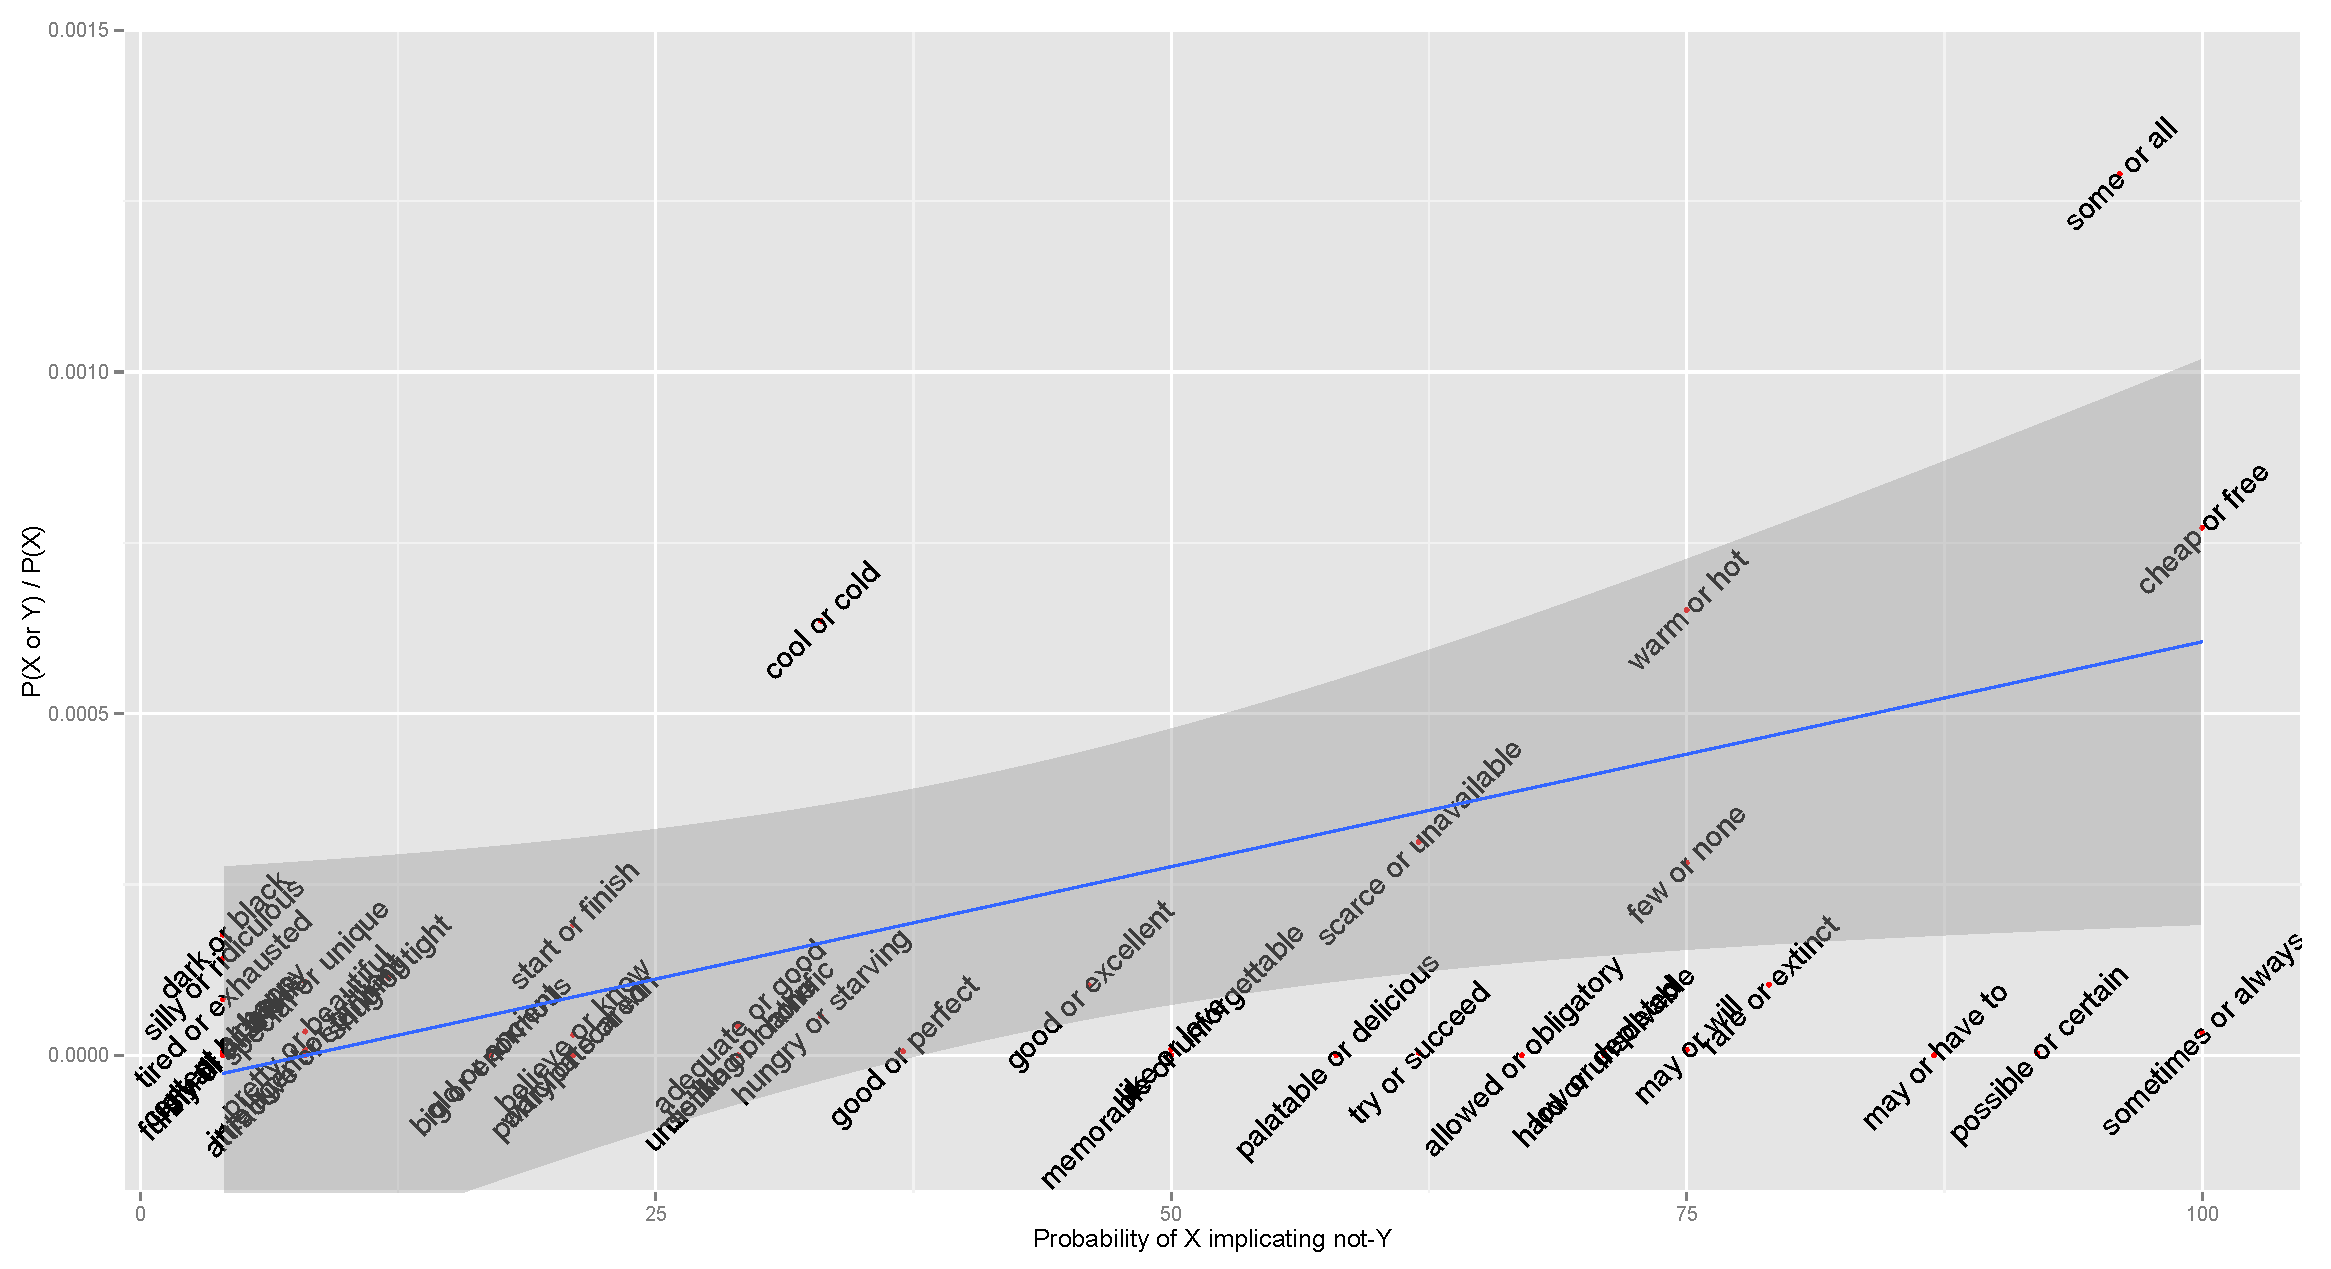
\includegraphics[width=1\textwidth]{fig/chemla}
  \caption{A corpus study inspired by \citet{Chemla-HurfordCounts} on
    the relationship between the probability that \word{X}
    conversationally implicates \word{not-Y} and the 
    frequency of disjunctions \word{X or Y} relative to 
    the more general term \word{X}. A linear regression (blue line)
    suggests a modest but robust correlation (coef = $6.580^{-06}$; 
    standard error $3.095^{-06}$; $p = 0.04$; $R^{2} = 0.08$).}
  \label{fig:chemla}
\end{figure}

The speaker might wish to block a subtly different kind of implicature
in a situation in which a general term is prone to being limited to a
prototypical subkind \citep{Levinson00}. For instance, at a busy
marina in water-skiing country, \word{boat} might come to identify
just motorboats. In that case, a speaker might use \word{boat or
  canoe} or \word{boat or kayak} to ensure that these non-motorized
cases are included in a rule, lest people assume that these rarer
kinds of boat are exempt.

In both of these implicature-blocking scenarios, the speaker is
concerned that the general term \word{X} will be construed as
$\sem{\word{X}}-\sem{\word{Y}}$ for some \word{Y}. Thus, \word{X} or
\word{Y} is a hedge against the possibility that the listener's view
of language is such that, at least in the current context,
$\sem{\word{X}} \cap \sem{\word{Y}} = \emptyset$, or, as in
\posscitet{Singh:2008} account,
$\sem{\word{Y}} \nsubseteq \sem{\word{X}}$. This is a defensive
position; the speaker's own lexicon might allow her to use just the
general term to convey her intentions, but she is concerned that the
listener will arrive at a different conclusion. The costs of
disjunction are therefore worth paying even if it adds no new
information given the speaker's lexicon.  However, the speaker can
play a more active role as well, using disjunctions to instruct the
listener about the right lexicon. Our \secref{sec:introduction}
example containing ``you may need angioplasty or surgery'' seems to be
an instance of this: the disjunction conveys secondary information
that \word{angioplasty} and \word{surgery} will be treated as separate
options in the current discourse. If HG were adopted as an explicit
theoretical constraint, then the possibility of doing this would more
or less follow --- we just require the additional premise that the
listener is charitable and so will try to find an acceptable construal
of the utterance. The model we develop in \secref{sec:model} also
supports this kind of reasoning, but it requires no independent
statement of HG.
 
%%%%%%%%%%%%%%%%%%%%%%%%%%%%%%%%%%%%%%%%%%%%%%%%%%%%%%%%%%%%%%%%%%%%%%

\subsection{Definition and identification}\label{sec:data:definitional}

% A Geological History of Manhattan or New York Island

Disjunctions like \word{wine lover or oenophile} seem to fly in the
face of the Hurfordian pressure reviewed just above. Rather than
avoiding overlap, they seem to embrace it, conveying something
approximating identity. These readings seem to be more contextually
restricted even than HG-violating disjunctions, and speakers often
(but not always) signal them with ad hoc prosody, italics, quotation
marks, and other devices. However, it would be a mistake to dismiss
them as an idiosyncracy of English, since these uses are widely
attested in typologically diverse languages (we have examples from
Chinese, German, Hebrew, Ilokano, Japanese, Russian, and
Tagalog). Even languages that seem to have a dedicated `definitional'
or `metalinguistic \word{or}' (e.g., Finnish, Italian) seem also to
allow the regular \word{or} to play this role.

For our purposes, the most important property of these uses is that
they convey a meaning that is secondary to the main content of the
utterance --- an extreme instance of a meaning that is not at issue
\citep{Tonhauser-etal:2011}. This contrasts with overt definitions
like \word{oenophile means wine-lover} or \word{oenophile: wine-lover}
(in a dictionary context).  We think it is no accident that another
strategy for conveying definitional information in this non-asserted,
taken-for-granted manner is via apposition, as in \word{oenophile
  (`wine-lover')} \citep{Potts05BOOK}. In this respect, the relevant
inference resembles the exclusivization pressure identified by HG:
both seem to emerge as side-effects rather than normal outputs. In our
model (\secref{sec:model}), both are in turn characterized as
inferences about the lexicon rather than about the state of the world.

In addition, as with disjunct exclusivization, the relevant lexical
inference might be temporary. For instance, phrases like
\word{Internet or computer network} seem to use the second phrase as a
rough-and-ready way of helping the listener bootstrap towards an
understanding of what the Internet is like. Even our wine-lover
example seems to involve only approximate synonymy; \word{wine lover
  or oenophile} seems apt in a context in which the speaker wishes to
use \word{oenophile} to elevate the concept to something more specific
(or pretentious) than \word{wine lover} picks out. Similarly, the book
title \emph{A Geological History of Manhattan or New York Island}
seems to identify Manhattan and New York Island while at the same time
acknowdging the different histories and connotations of the two
disjunct terms.

The speaker's motivations for using definitional disjunction are quite
varied. Such readings seem to arise most easily when the speaker is
mutually and publicly known to be a expert in the domain covered by
the terms and the listener is mutually and publicly known to be
inexpert in that area. In such cases, the speaker can use the
disjunction to convey information about her preferred lexicon, fairly
certain that the listener will be receptive. However, while speaker
expertise seems to be a genuine prerequisite, the listener's knowledge
seems to impose much less.  We find natural uses of this strategy when
there is no direct information about the listener, but rather just a
general assumption that one of the terms is relatively unknown. For
instance, a newspaper article might contain \word{wine lover or
  oenophile} without presuming that all its readers are ignorant;
rather, such a use would seem to presuppose only that \word{oenophile}
is relatively unknown.  Finally, at the the other end of the extreme,
the listener might actually be presumed to know the term, but the
speaker sees social value in conveying that she shares this view. This
could be because the speaker would like to display expertise, as when
an ambitious undergraduate seeks to convey competence to a professor.
The uses also arise when the speaker and listener might both be
experts in the domain and see a value (jointly or just in the current
speaker's eyes) of using a word in a specialized sense in order to
name a concept efficiently (e.g., \word{What motivates the snobbish
  wine lover or `oenophile' and how does he differ from the casual
  drinker?}).

For these reasons, we retreat to a more basic characterization: the
discourse participants must have a mutual interest in communicating
about their language and arriving at a refined, perhaps
context-specific joint understanding of it, and there should be a
background assumption that speaker and listener are willing to
coordinate on the lexicon that the speaker seems to be using. In
addition, we hypothesize that the cost of using a disjunction must be
fairly small, all things considered, else it is hard to see how the
speaker could justify using a disjunction \word{X or Y} to convey
simply $\sem{\word{X}}$. At any rate, whatever the costs of using the
verbose form, they must be worth paying in virtue of the benefits of
identifying (for the purposes of the current talk exchange) the
meanings of the two disjuncts.

% There can be uncertainty about whether the listener should regard
% the disjunction as definitional. We might enter into a blurry area
% in which the listener is struggling to figure out whether the
% intentions are definitional or exclusivizing. This can persist even
% when one of the words is unknown to the listener. In such cases, the
% disjunctive meaning is just extremely general and will not do
% justice to the speaker's intentions.


%%%%%%%%%%%%%%%%%%%%%%%%%%%%%%%%%%%%%%%%%%%%%%%%%%%%%%%%%%%%%%%%%%%%%%

\section{Modeling communication with anxious experts}\label{sec:model}

We now present our model of pragmatic reasoning. Our presentation is
somewhat compact. Readers wishing to more fully explore the model are
referred to the website for this paper, which implements the model,
provides simple and complex examples, and includes (Python) code for
all the examples and figures in this paper.

In our model, production and interpretation are based in a recursive
process in which speaker and listener agents reason about each other
reasoning about each other.  At the lowest levels of our model, these
agents communicate using a single lexicon. However, we do not actually
assume that a single lexicon is mutually and publicly recognized as
the set of core conventions of the language. Rather, our model
aggregates over many possible lexica, thereby allowing the agents to
negotiate the structure of the language itself even as they
communicate. \Figref{fig:modstruc} summarizes this picture
schematically; this section is devoted to explicating these agents and
their relationships.

\begin{figure}[tp]
  \centering
  \newcommand{\labelednode}[2]{\put(#1){\makebox(0,0){#2}}}
  \newcommand{\picarrow}[3][0.9]{\put(#2){\vector(#3){#1}}}
  \newcommand{\picdownarrow}[1]{\picarrow{#1,0.8}{3,-2}}
  \newcommand{\picuparrow}[1]{\picarrow{#1,0.2}{3,2}}
  \setlength{\unitlength}{1cm}
  \begin{picture}(8,1.5)
    \labelednode{1,1.5}{\textbf{Fixed $\Lex$}}
    \labelednode{5.5,1.5}{\textbf{Reasoning about possible $\Lex$}}
    \labelednode{0,1}{$\listenerZero$}
    \picdownarrow{0}
    \labelednode{1,0}{$\speakerOne$}
    \picuparrow{1}
    \labelednode{2,1}{$\listenerOne$}
    \picarrow[0.7]{2.1,1}{1,0}
    \labelednode{3,1}{$\ListenerK[1]$}
    \picdownarrow{3}
    \labelednode{4,0}{$\SpeakerK[2]$}
    \picuparrow{4}
    \labelednode{5,1}{$\ListenerK[2]$}
    \picdownarrow{5}
    \labelednode{6,0}{$\SpeakerK[3]$}
    \picuparrow{6}
    \labelednode{7,1}{$\ListenerK[3]$} 
    \picdownarrow{7}
    \labelednode{8,0}{$\ldots$}
  \end{picture}
  \caption{Summary of model structure.}
  \label{fig:modstruc}
\end{figure}

The core structures of our model are given in \eg{model}.
Intuitively, we imagine that a speaker and listener are playing a game
in which the speaker privately observes a state $\state \in \States$
and produces a message $\msg \in \Messages$ on that basis, given the
context defined by the signaling system. The listener then uses $\msg$
to guess a state $\state' \in \States$, and the communication succeeds
just in case $\state = \state'$. The agents that we define are
rational in the sense that, by reasoning recursively about each
other's behaviors, they can increase their chances of success at this
signaling game.
%
\begin{examples}
\item\label{model}
  \begin{examples}
  \item\label{states}%
    $\States$ is a set of states (worlds, referents, propositions, etc.).
  \item\label{messages}%
    $\Messages$ is a set of messages containing designated `null' message $\nullmsg$.
  \item\label{lex}%
    $\Lex: \Messages \mapsto \wp(\States)$ is a semantic interpretation function. 
    $\Lex'(\nullmsg) = \States$.
  \item\label{prior}%
    $\Prior : \States \mapsto [0,1]$ is a prior probability
    distribution over states.    
  \item\label{costs}%
    $\Costs : \Messages \mapsto \Reals$ is a cost function on messages.
    $\Costs(\nullmsg) > \Costs(\msg), {\forall \msg \in \Messages{-}\set{\nullmsg}}$.
  \end{examples}
\end{examples}

Clause~\subeg{model}{messages} designates a null message $\nullmsg$
that is true in all states in all lexica. It can be thought of as a
catch-all for the numerous messages in the language that are not
discriminating in the context defined by the signaling system.  No
matter how big and complex the examples, such a message is always
justified. Introducing $\nullmsg$ also helps ensure that various
calculations in the model are well-defined. (For alternative methods
of ensuring definedness, see \citealt{Jaeger:2011} and
\citealt{bergen-levy-goodman:2014}.)

%=====================================================================

\subsection{Simple state/message signaling}\label{sec:rsa}

As \figref{fig:modstruc} shows, our model defines an intuitive hierarchy
of agents. The most basic are $\listenerZero$, $\speakerOne$, and
$\listenerOne$. These agents reason in terms of a fixed lexicon
$\Lex$, which, for our purposes, can be thought of as a standard
semantic interpretation function, as in \subeg{model}{lex}. These
agents suffice to define a version of the Rational Speech Acts model
of \citet{Frank:Goodman:2012} and \citet{Goodman:Stuhlmuller:2013}.

The starting point is $\listenerZero$. This agent simply turns $\Lex$
into a probabilistic formulation that can be used for decision-making
in the presence of communicative indeterminacy. The first term just
defines an even distribution over all of the true states $\state$ for
the given message $\msg$, and the second term incorporates the
contextual prior distribution over states $\Prior$.
%
\begin{examples}
\item\label{l0}%
  $\listenerZero(\state \given \msg, \Lex) \propto
  \frac{\Indicator(\state \in \Lex(\msg))}{|\Lex(\msg)|}
  \Prior(\state)$
\end{examples}

This agent is pragmatic only insofar as it incorporates the contextual 
prior into (a distribution derived from) the truth conditions. Richer
pragmatic inferences start to emerge as soon as we envision a speaker
who can reason in terms of this listener and plan its utterances 
accordingly. The minimal such speaker is $\speakerOne$, which is 
defined recursively in terms of $\listenerZero$:
%
\begin{examples}
\item\label{s1}% 
  $\speakerOne(\msg \given \state, \Lex) \propto
  \exp
  \left(
    \log\left(\alpha\,\listenerZero(\state \given \msg, \Lex) \right)
    - 
    \gamma\,\Costs(\msg)
  \right)$
\end{examples}
%
Ths definition is a bit cumbersome because of the need to ensure that
all values are positive. At its heart, though, this agent is parallel
to $\listenerZero$ in that it just combines a conditional distribution
and a piece of contextual information --- now costs on messages. The
result is a distribution that one can imagaine serving as the basis
for decision making: given that the agent would like to convey that a
certain state holds, which message will do that most effectively for
the $\listenerZero$ listener? The real-valued parameter $\alpha$
controls the degree to which the speaker tries to capitalize on the
distinctions encoded by $\listenerZero$.

The first pragmatic listener is $\listenerOne$. It is parallel to
$\listenerZero$ except that it reasons, not in terms of the original
lexicon, but rather in terms of $\speakerOne$ reasoning about
$\listenerZero$ reasoning about the lexicon. This gives rise to a
derive, pragmatically-enriched probabilistic interpretation function.
%
\begin{examples}
\item\label{l1}% 
  $\listenerOne(\state \given \msg, \Lex) \propto 
  \speakerOne(\msg \given \state, \Lex)
  \Prior(\state)$
\end{examples}

\Figref{fig:rsa-disj} shows how this model derives a basic scalar
implicature. We've used disjunction to illustrate, but the reasoning
is actually general across all instances in which a general term $X$
competes with a specific subterm $Y$. In terms of the communication
game, suppose the speaker's private state is $w_{2}$. The literal
listener $\listenerZero$ has only a 50/50 chance of identifying this
state given the message $\porq$.  However, the first pragmatic
listener $\listenerOne$, reasoning in terms of $\speakerOne$, has
already learned to separate $\porq$ and $\pandq$. The nature of
$\speakerOne$ is equally interesting, as it has achieved a
production-oriented version of the scalar implicature, as a bias for
producing $\pandq$ where it is true.

This basic model has been shown to achieve good quantitative fits to
experimental results
\citep{Degen:Franke:2012,Stiller:Goodman:Frank:2011}. One can also
generalize $\listenerOne$ and $\speakerOne$ to allow them to
recursively respond to each other. This has the effect of soldifying
implicatures, but it seems also to predict complex ones that speakers
are less inclined to perceive \citep{Vogel-etal:2014}.

\begin{figure}[tp]
  \centering
  \setlength{\arraycolsep}{3pt} 
  $\begin{array}[b]{c c r@{\hspace{25pt}}l}
     \listenerMatrix%
     {\Lex_{1}}%
     {\True & \True  & \False}
     {\True & \False & \False}     
     {\True & \True  & \True}      
     &
     \rightarrow
     &
     \listenerMatrix%
     {\listenerZero}%
     { .5  &  .5 & 0}%
     {  1 &   0 &  0}%
     {.33 & .33 & .33}%
     &
     \listenerMatrix%
     {\listenerOne}%
     {.25 & .75 & 0}%
     {1 &   0 & 0}%
     { 0 &   0 & 1}
   \\
   && \searrow & \nearrow
   \\
   &&
   \multicolumn{2}{c}{
      \speakerMatrix%
      {\speakerOne}%
      {.33 & .67 & 0}%
      {1 &   0 & 0}%
      {0 &   0 & 1}
   }
   \end{array}$   
   \caption{Illustrating simple state/message signaling with
     disjunction.  We assume an even prior over states and $0$ costs
     for all messages. The recursive process separates disjunction
     (general) and conjunction (specific), thereby creating a pattern
     characterizable as a scalar implicature.}
  \label{fig:rsa-disj}
\end{figure}

%=====================================================================

\subsection{Lexical uncertainty and expertise}\label{sec:full}

In the above simple mode, the agents condition on (take as given) a
fixed, shared lexicon. Howver, the data in \secref{sec:data} show that
the lexicon is not known precisely, but rather negotiated during
interactions. We now bring that insight into our model. The first step
is to define a space of lexica $\LexSet$ and a probability
distribution over them $\LexPrior$:
%
\begin{examples}
\item\label{model-extend}
  \begin{examples} 
  \item\label{lexset}%
      $\LexSet = \set{\Lex' : \Lex'(\nullmsg) = \States \text{ and } 
      \forall \msg \in \Messages{-}\set{\nullmsg}, 
      \Lex'(\msg) \neq \emptyset \text{ and } 
      \Lex'(\msg) \subseteq \Lex(\msg)}$
  \item\label{LexPrior}% 
    $\LexPrior : \LexSet \mapsto [0,1]$ is a prior
    probability distribution over lexica.  
  \end{examples}
\end{examples}
%
Clause~\subeg{model-extend}{lexset} defines a complete set of
refinements of a basic lexicon: every lexical item can denote a subset
of the space it denotes in the focal lexicon $\Lex$, and all
combinations of these refinements are available. The only requirements
are that messages always have non-empty denotations and that the null
message $\nullmsg$ always denotes the full set of states. The
resulting definition gives us an intuitive, computationally manageable
space to work with. We should emphasize, though, that these
assumptions are not essential to our model. In the extreme case, we
could admit every lexicon derivable from the messages $\Messages$ and
states $\States$, and then usee the lexicon prior $\LexPrior$ to
provide some structure to the space --- say, but assigning low but
non-zero probability to lexica that are not refinements. This is a
strictly more general perspective than the one given by
\eg{model-extend}, which can alternatively be seen assigning zero
probability to lexica not admitted by
clause~\subeg{model-extend}{lexset}. We do not explore these options
further in this paper, but see for discussion of non-refinement
pragmatic enrichment.

\Figref{fig:disjlexica} shows the set of admissible lexica for the
initial lexicon $\Lex$ of \figref{fig:rsa-disj}. Since $\pandq$
already denotes a singleton, it admits no refinements, so its meaning
is the same in all three lexica. The null message $\nullmsg$ is fixed
by stipulation. The message of interest is disjunction, since it has
two refinements in addition to its basic meaning. Even in this simple
example, one can see how useful biases will start to emerge. For
instance, $\porq$ has two lexica in which its meaning includes
$w_{2}$, but just one in which it includes $w_{1}$. This bias is
already pushing in the direction of the target pragmatic association
of $\porq$ with $w_{2}$ that we see for $\listenerOne$ in
\figref{fig:rsa-disj}.

\begin{figure}[tp]
  \centering
  \setlength{\arraycolsep}{1pt}    
  $\begin{array}[c]{c c c}
     \Lex & \Lex_{2} & \Lex_{3} \\
     \disjlexicon{w_{1}, w_{2}}{w_{1}}
     & 
     \disjlexicon{w_{1}}{w_{1}}
     & 
     \disjlexicon{w_{2}}{w_{1}}
  \end{array}$
  \caption{Lexicon set $\LexSet$ for the basic lexicon $\Lex$ in \figref{fig:rsa-disj}.}
  \label{fig:disjlexica}
\end{figure}

Our first `lexical uncertainty' agent is $\ListenerK[1]$, which is based
on the model of \citet{Smith:Goodman:Frank:2013}:
%
\begin{examples}
  \item\label{L1}%
    \setlength{\arraycolsep}{2pt}%  
    $\mspace{-4mu}\begin{array}[t]{r c l}
      \ListenerK(\state, \Lex \given \msg) 
      &=&
      \ListenerK(\state \given \msg, \Lex) \ListenerK(\Lex \given \msg) 
      \\[1ex]
      \ListenerK(\Lex \given \msg) 
      &\propto& 
      \Prior(\Lex) \sum_{\state\in\States} \SpeakerK(\msg \given \state, \Lex)\Prior(\state)
    \end{array}$
\end{examples}
%
This agent is defined for levels $k \geqslant 1$ as long as we assume
that $\SpeakerK[1] = \speakerOne$ (higher levels use the speaker in
\eg{Sk}) and
$\ListenerK[1](\state \given \msg, \Lex) = \listenerOne(\state
\given \msg, \Lex)$.
The agent uses the speaker's message to make a joint inference about
the state and the lexicon. The first term uses a fixed-lexicon
inference and the second encodes the extent to which the current
message biases in favor of $\Lex$.

Our `expertise' speaker responds to this lexical uncertainty listener.
We assume that this speaker does have a specific lexicon in mind.  More
precisely, this speaker is taken to observe state--lexicon pairs and
produce messages on that basis. It is defined for all $k > 1$:

\begin{examples}  
  \item\label{Sk}%
    $\SpeakerK(\msg \given \state, \Lex) \propto 
    \exp
    \left(
      \log
      \left(\alpha\,\ListenerK[k-1](\state \given \msg, \Lex)\right)
      - 
      \beta \log\left(\ListenerK[k-1](\Lex\given\msg)\right)
      -
      \gamma\,\Costs(\msg)
    \right)$
\end{examples}
%
In broad terms, this agent is similar to $\speakerOne$ except that it
includes a new term $\ListenerK[k-1](\Lex\given\msg)$ encoding the
information each message conveys about the lexicon. The relative
importance of this information is controlled by a new real-valued
learning-rate parameter $\beta$. The relative weights of $\alpha$ and
$\beta$ control the relative importance of conveying information about
the world and information about the lexicon, and much of our
investigation of disjunction focuses on this relationship.

\Figref{fig:full-disj} shows this model in action on our simple
disjunctive scalar implicature. The left column gives the
$\listenerOne$ inferences for the three lexica in
\figref{fig:disjlexica}. The middle column gives the uncertainty
listener's joint probabilities given each message. It says, for
example that the listener's best-guess (highest probability) inference
given the message $\porq$ is state $w_{2}$ and lexicon $\Lex_{1}$ or
$\Lex_{3}$. The right column shows the first expertise speaker's
message probabilities given observed state--lexicon pairs. From here,
the iteration between $\ListenerK[k-1]$ and $\SpeakerK$ could continue.

\marginpar{I'm confused about why speaker uses $\porq$ in $\Lex_{1}/w_{2}$, where it is false!}

\begin{figure}[tp]
  \centering
  $\begin{array}{c c c}
     \listenerOne & \ListenerK[1] & \SpeakerK[2] 
     \\[1ex]     
     \listenerMatrix%
     {\Lex_{1}}%
     {.25 & .75 & 0}%
     {1 & 0 & 0}%
     {0 & 0 & 1}     
     &
     \ListenerKMatrix%
     {\porq}%
     {.12 & .35 & 0}%
     {.18 & 0 & 0}
     {0 & .35 & 0}            
     &
     \SpeakerKMatrix%
     {1}%
     {.31 & .69 & 0}%
     {1 & 0 & 0}%
     {0 & 0 & 1}
     %
     \\[8ex]
     %
     \listenerMatrix%
     {\Lex_{2}}%
     {1 & 0 & 0}%
     {1 & 0 & 0}%
     {0 & .5 & .5}%
     &
     \ListenerKMatrix%
     {\pandq}%
     {.31 & 0 & 0}
     {.23 & 0 & 0}
     {.46 & 0 & 0}
     &
     \SpeakerKMatrix%
     {2}%
     {.18 & .82 & 0}%
     {.99 & 0 & .01}%
     {0 & 0 & 1}%       
     %
     \\[8ex]
     %
     \listenerMatrix%
     {\Lex_{3}}%
     {0 & 1 & 0}%
     {1 & 0 & 0}%
     {0 & 0 & 1}%
     &
     \ListenerKMatrix%
     {\nullmsg}%
     {0 & 0 & .25}%
     {0 & .25 & .25}%  
     {0 & 0 & .25}%
     &
     \SpeakerKMatrix%
     {3}%
     {.18 & .82 & 0}%
     {1 & 0 & 0}%
     {0 & 0 & 1}%  
   \end{array}$
   \caption{Full model inferences for disjunction. $\alpha = 1$
   $\beta = 1$. $\Costs(\nullmsg) = 5$.}
  \label{fig:full-disj}
\end{figure}

%=====================================================================

\subsection{A return to simple signaling}\label{sec:return}

The full model can be unwieldy to think about because of the lexicon
inferences. To return to the intuitive picture of simple state/message
signaling, we can sum over lexica, as in \eg{lisnorm} and
\eg{spknorm}. Both provide useful summaries of the model's
predictions. \Figref{fig:simple} by using these equations to reduce
the middle and right columns of \figref{fig:full-disj} to just 
state/message relationships. The results closely match those obtained
from the simpler system (\figref{fig:rsa-disj}).
%
\begin{examples}
\item\label{lisnorm}% 
  $\ListenerK(\state \given \msg)  = 
  \sum_{\Lex \in \LexSet} \ListenerK(\state, \Lex \given \msg)$
\item\label{spknorm}% 
  $\SpeakerK(\msg \given \state) \propto 
  \sum_{\Lex \in \LexSet} \SpeakerK(\msg \given \state, \Lex)
  \LexPrior(\Lex)$
\end{examples}

\begin{figure}[tp]
  \centering
  $\begin{array}[c]{c@{\hspace{45pt}}c}
     \ListenerK[1](\state\given\msg) & \SpeakerK[2](\msg\given\state) \\[1ex] % & \ListenerK[2](\state\given\msg) \\[1ex]
     \listenerMatrix%
     {}%
     { 0.29 & .71 & 0}
     { 1 &   0 &  0}
     {0 &  .25 & .75}
     & 
     \speakerMatrix%
     {}%
     {.23 &  .77  &   0}%
     {1   &  0  &     0}%
     {0   &  0  &   1}
     %
     % & 
     %
     %\listenerMatrix%
     %{}
     %{ .18 & .82  &  0}
     %{1 &   0  &  0}   
     %{0 &   0  &  1}      
   \end{array}$
   \caption{A return to simple signaling. The system on the left is
     derived from the middle column of \figref{fig:full-disj} using
     equation~\eg{lisnorm}, and the right column is derived from the
     right column of \figref{fig:full-disj} using
     equation~\eg{spknorm}.}
  \label{fig:simple}
\end{figure}

%%%%%%%%%%%%%%%%%%%%%%%%%%%%%%%%%%%%%%%%%%%%%%%%%%%%%%%%%%%%%%%%%%%%%%

\section{Compositional disjunction}\label{sec:composition}

The running example we used in \secref{sec:model} to introduce the
model is artificial and overly simplisitic in a bunch of ways, the
most glaring of which is its noncompositional treatment of disjunction
(and conjunction). Since this paper is largely about disjunction, it's
important that we get somewhat more serious about that aspect of the
messaging system.

To achieve this, we begin from a space of atomic messages and close
them under disjunction. So, for example, $\set{p, q}$ expands to
$\Messages = \set{p, q, \porq, \pandq}$. In addition, in order to
directly model the sort of indeterminacy that disjunction can convey,
we close the set of atomic states under the join operation.  For the
set of atomic states $\set{w_{1}, w_{2}, w_{3}}$, this results in the
semilattice in \figref{fig:closure}. Interpretation via $\Lex$ then
proceeds as one would expect: disjunction corresponds to union and
conjunction to intersection. For example, if $p$'s meaning is
$\set{w_{1}, w_{2}}$ and $q$'s meaning is $\set{w_{1}, w_{3}}$, then
$\porq$ denotes $\set{w_{1}, w_{2}, w_{3}}$.  After join closure, this
denotes the entire state space represented in
\figref{fig:closure}. Conversely, $\pandq$ denotes $\set{w_{1}}$,
which does not change under closure. (We expand the space of meanings
to include meets, or even to the full double-set lattice with states
like $w_{1} \vee (w_{2} \wedge w_{3})$, as in
\citealt{levy-pollard:2001}, but we stick with the join space to keep
the presentation as simple as possible.)

\marginpar{Add notes on exploring $\alpha$.}

\Figref{fig:compdisj} shows what happens when we run our full model
beginning from atomic messages $\set{p,q}$ and atomic states
$\set{w_{1}, w_{2}, w_{3}}$. The barplots summarize the
$\ListenerK[3]$ and $\SpeakerK[3]$ inferences using \eg{lisnorm} and
\eg{spknorm} to return to simple state/message signaling. The results
again reveal the expected exclusivization inferences for disjunction.

\begin{figure}[tp]
  \centering
  \newcommand{\labelednode}[2]{\put(#1){\makebox(0,0){#2}}}
  \newcommand{\picline}[3]{\put(#1){\line(#2){#3}}}
  \setlength{\unitlength}{1cm}
  \begin{picture}(5.5,2)   
    \labelednode{0.5,2}{$w_{1}$}
    \labelednode{2.75,2}{$w_{2}$}
    \labelednode{5,2}{$w_{2}$}
    
    \picline{0.5,1.2}{0,1}{0.6}
    \picline{0.75,1.2}{3,1}{1.8}
    \labelednode{0.5,1}{$w_{1} \vee w_{2}$}
        
    \picline{2.5,1.2}{-3,1}{1.8}
    \picline{3.0,1.2}{3,1}{1.8}
    \labelednode{2.75,1}{$w_{1} \vee w_{3}$}

    \picline{5,1.2}{0,1}{0.6}
    \picline{4.75,1.2}{-3,1}{1.8}
    \labelednode{5,1}{$w_{2} \vee w_{3}$}
    
    \picline{2.5,0.2}{-3,1}{1.8}
    \picline{2.75,0.2}{0,1}{0.6}
    \picline{3.0,0.2}{3,1}{1.8}
    \labelednode{2.75,0}{$w_{1} \vee w_{2} \vee w_{3}$}
  \end{picture}
  \caption{State space with disjunctive closure.}
  \label{fig:closure}
\end{figure}

\begin{figure}[tp]
  \begin{subfigure}{0.48\textwidth}
    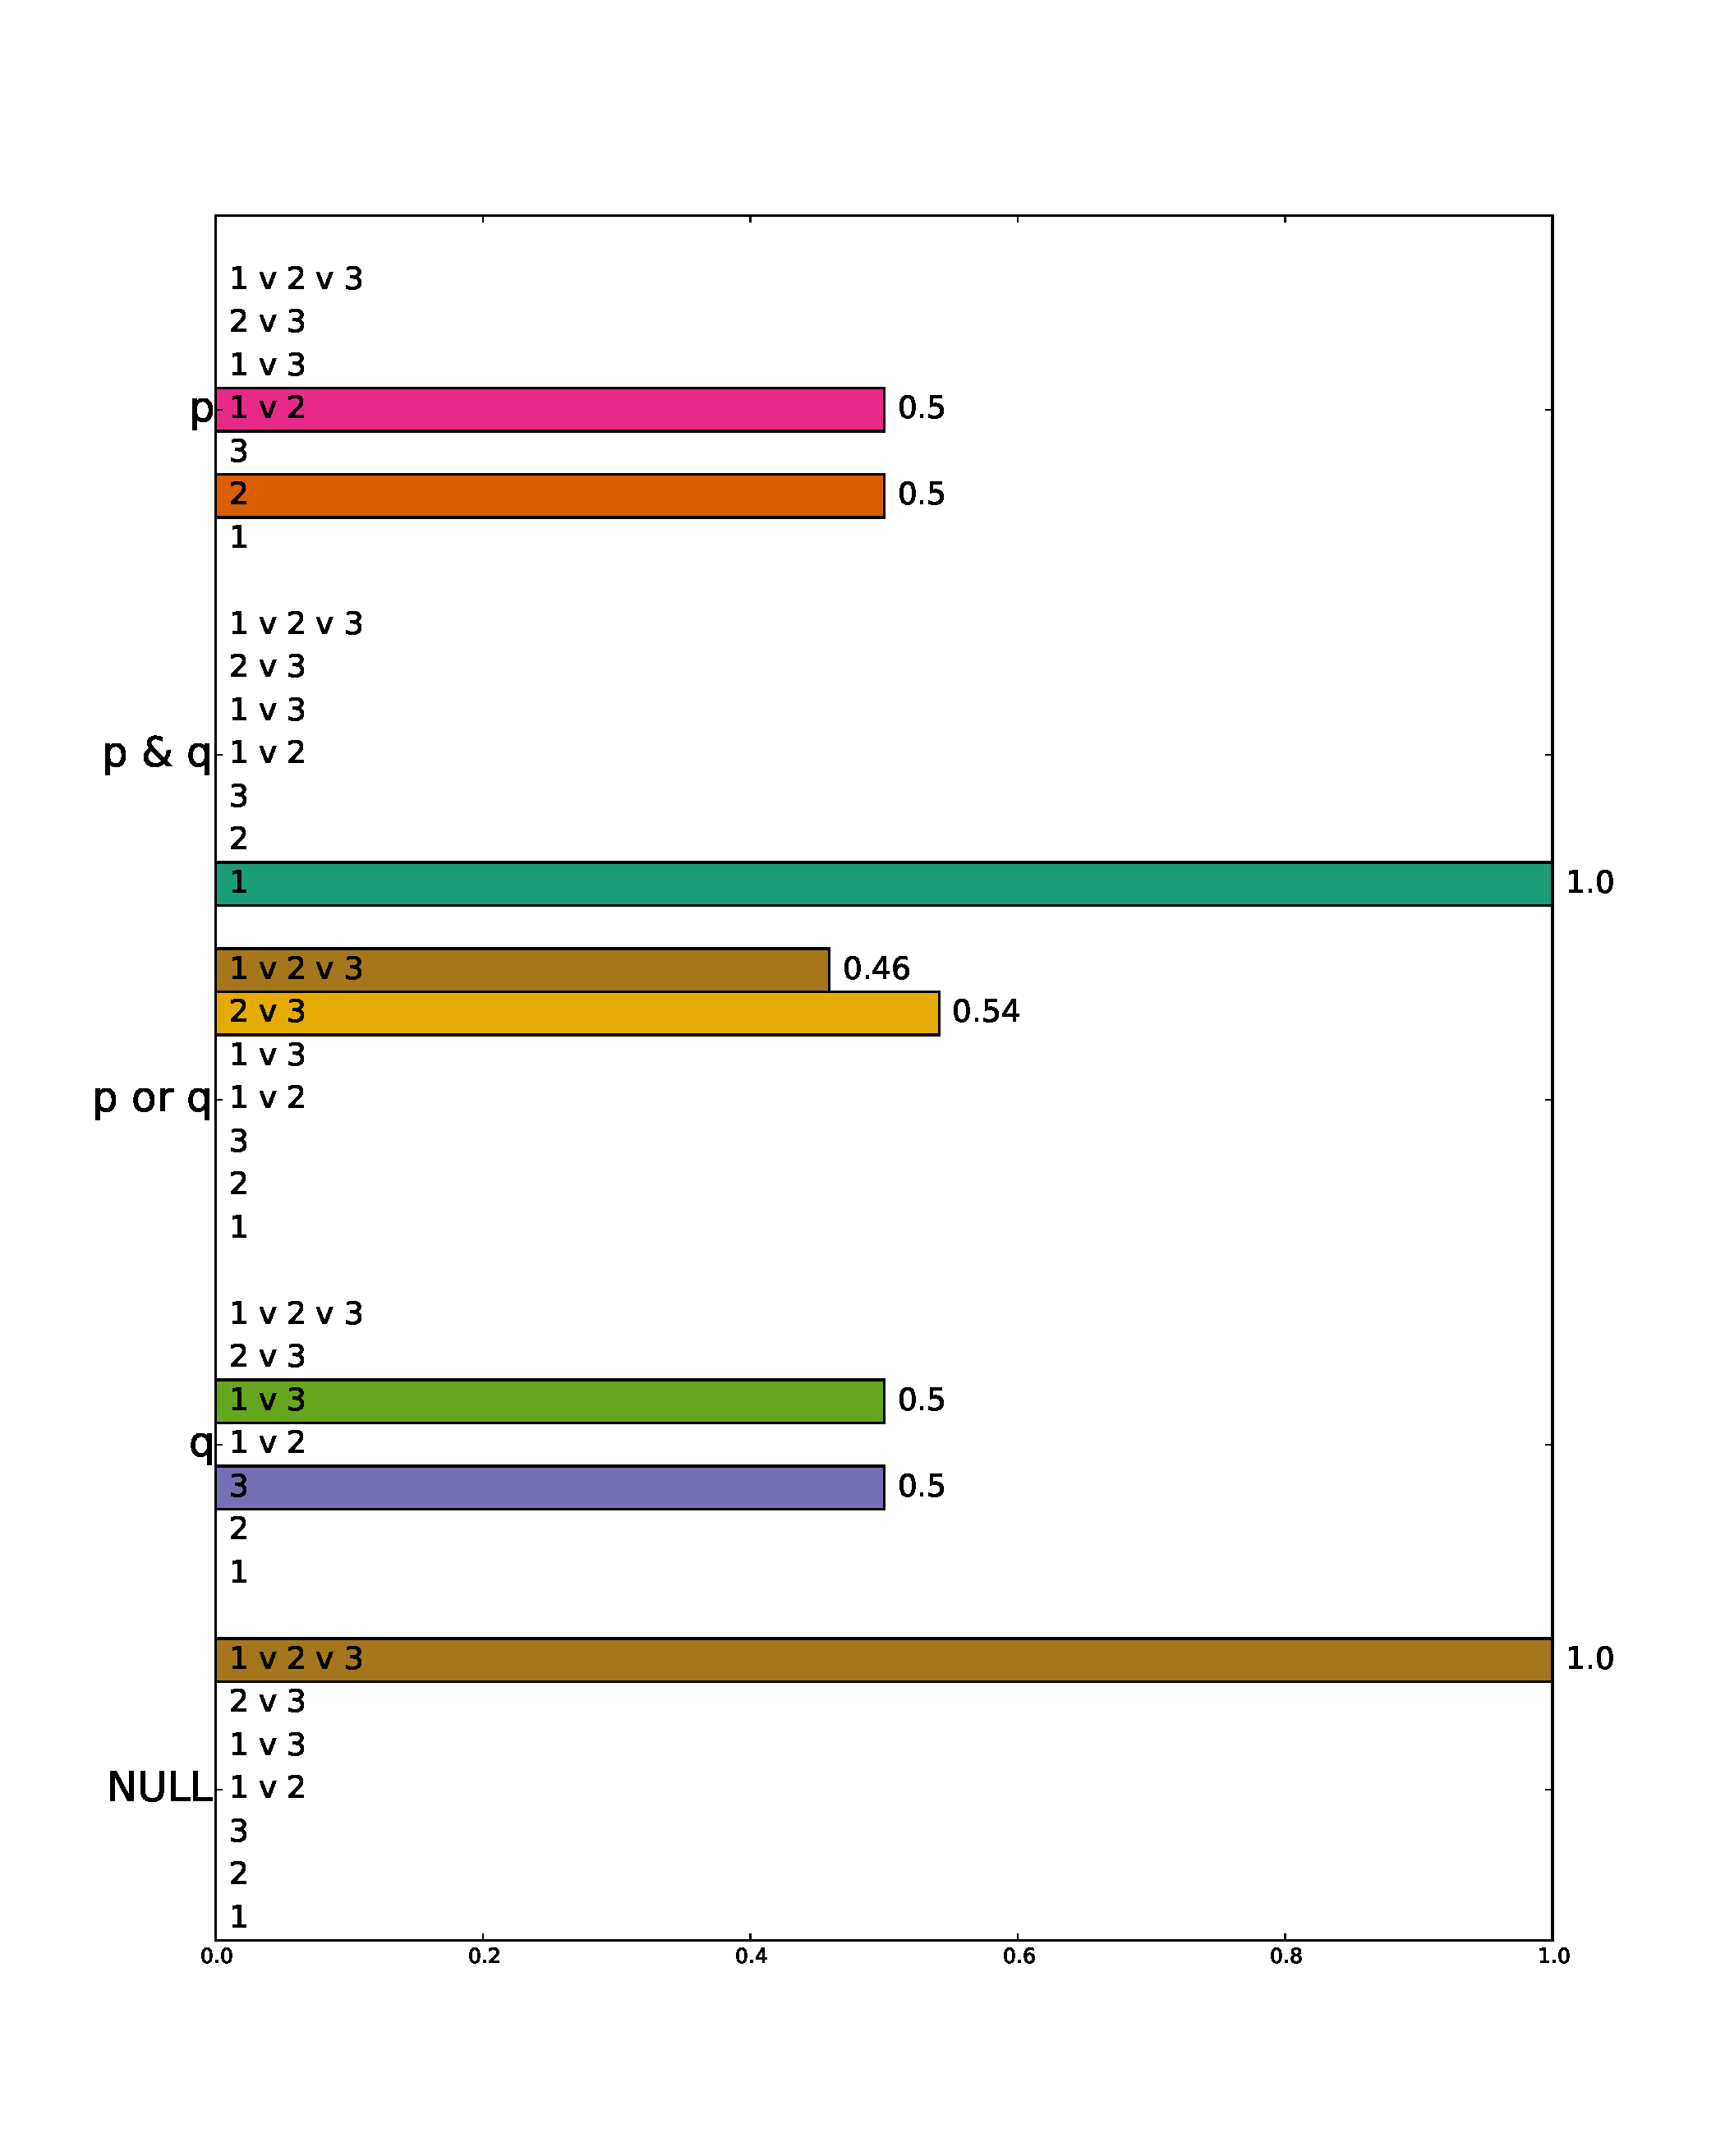
\includegraphics[width=1\textwidth]{fig/scalardisj-expertise-listener-marginalized}
  \end{subfigure}
  \hfill
  \begin{subfigure}{0.48\textwidth}
    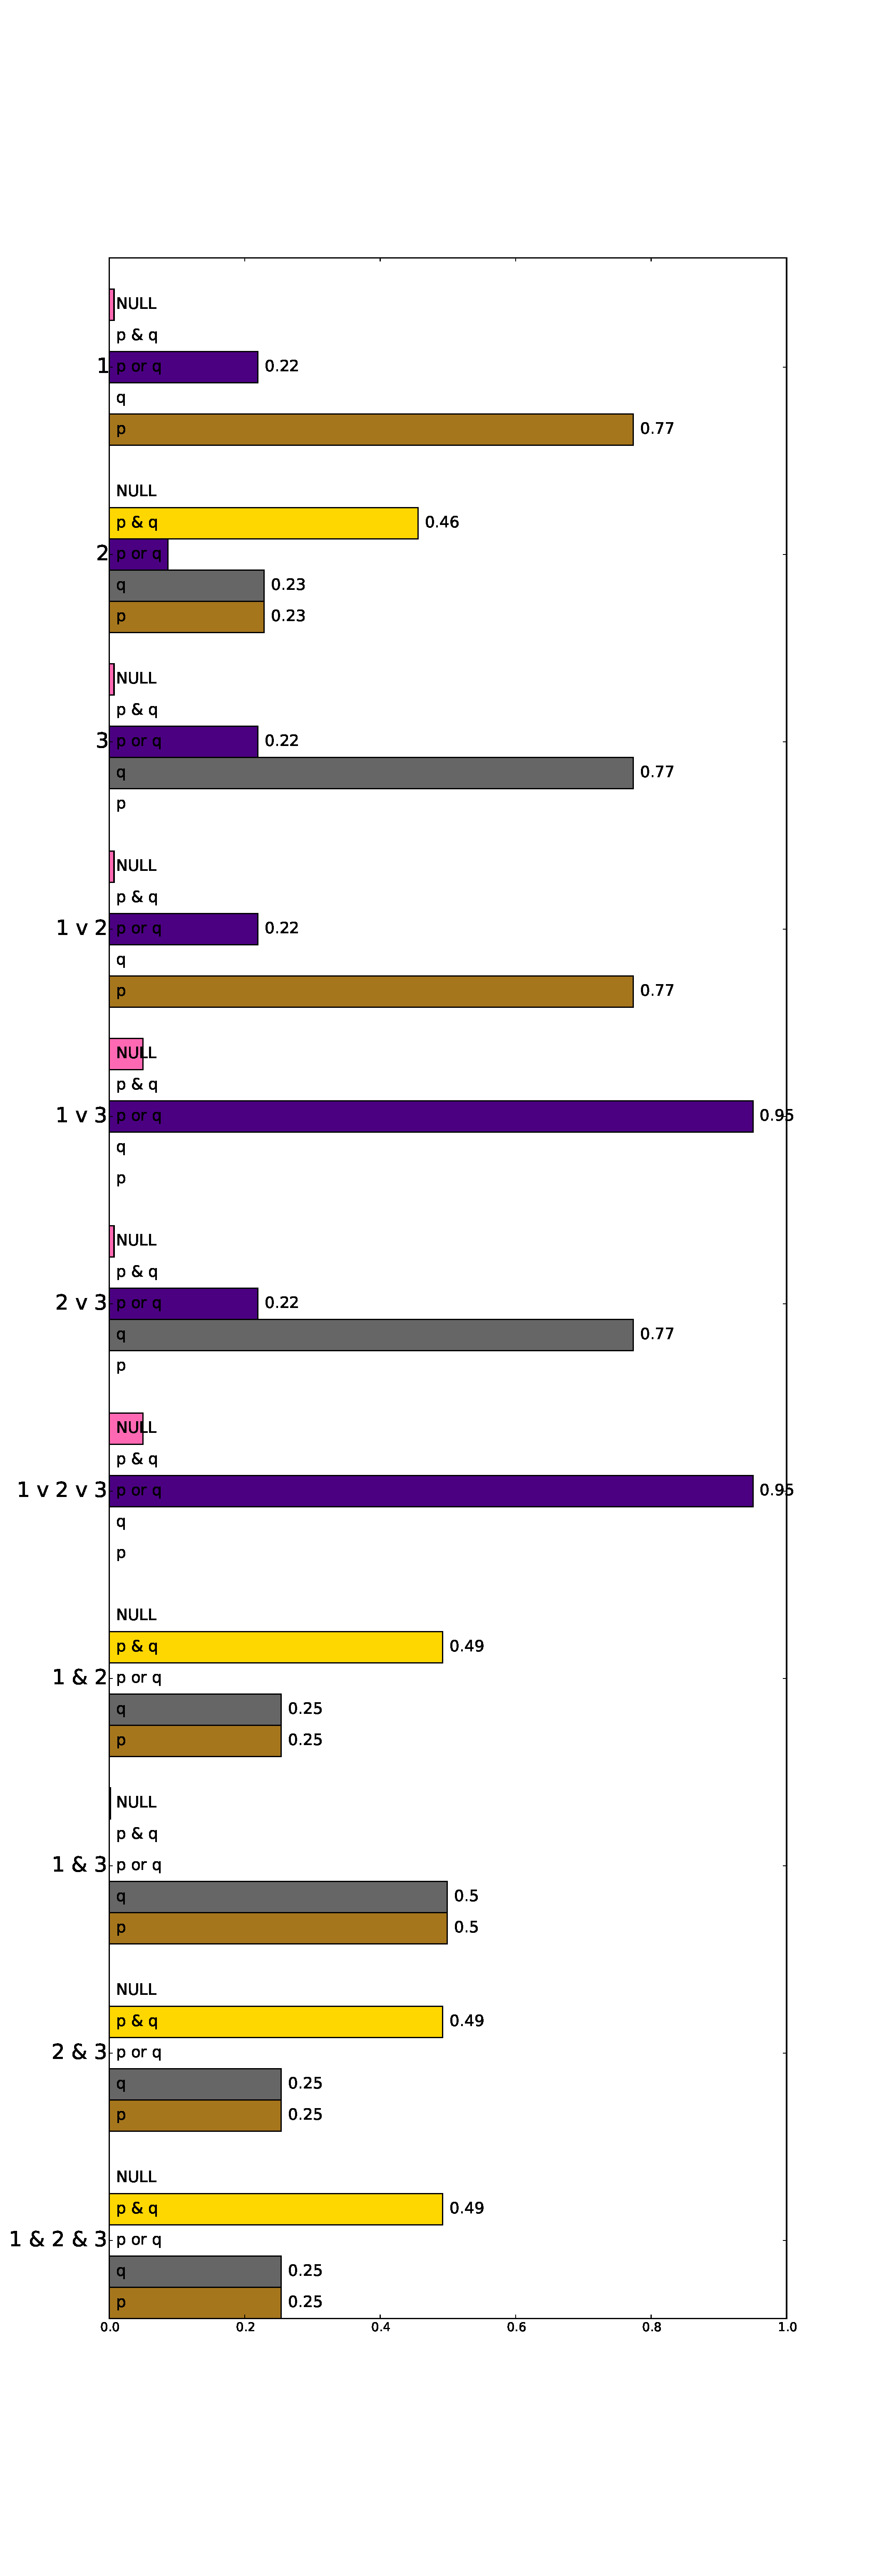
\includegraphics[width=1\textwidth]{fig/scalardisj-expertise-speaker-lexsum}
  \end{subfigure}
  \caption{Compositional disjunction results. $\alpha = 3$; $\beta = 1$; $\Costs(\vee) = 1.0$; $n = 10$}
  \label{fig:compdisj}
\end{figure}

\marginpar{\Figref{fig:compdisj} plots do not look good. I will work on them.}


%%%%%%%%%%%%%%%%%%%%%%%%%%%%%%%%%%%%%%%%%%%%%%%%%%%%%%%%%%%%%%%%%%%%%%

\section{Analysis}\label{sec:analysis}

We now show how our model can be used to characterize both the
Hufordian and definitional capacities of disjunction, as reviewed in
\secref{sec:data}. We first illustrate the effects using parameters
chosen by hand, and then we explore the space of parameters to try to
determine which settings --- which approximations of the context ---
deliver each of the readings. 

Throughout, our illustrations, we assume that \word{X} is the target
for refinement, that is, the general term for Hurfordian inferences
and the unknown term for definitional ones.  From the listener's
perspective, we are concerned to see when \word{A or X} gives rise to
the inference that $\sem{A} \cap \sem{X} = \emptyset$ (Hurfordian
reading) and when \word{A or X} gives rise to the inference that
$\sem{A} = \sem{X}$ (definitional).

It's worth highlighting again the dynamics of the model that
facilitate these uses. First, we assume that the speaker has a
preferred lexicon, and that she will choose her messages in part to
help convey this preference. Of course, the recusive nature of the
model means that the listener (or, rather, the speaker's expectations
about the listener) are involved in this planning. Second, we assume
that the listener is at least somewhat willing to defer to the speaker
with regard to the best lexicon to use in context. Again, this
deference is mediated by the recursive nature of the model, which
defines all aspects of communication as a (boundedly) rational
collaborative. We take these basic assumptions to be necessary, but
not sufficient, for communicating in language about language.

In our model, the importance of lexical communication is set by the
parameter $\beta$. If this is set to $0$, then all lexical preferences
are silenced. Where $\beta$ is positive, the ratio of $\alpha$ and
$\beta$ is a rough guide to the relative importance of communicating
about the world and communicating about the lexicon (though message
costs and other facts about context will also play a role).

%=====================================================================

\subsection{Hurfordian contexts}\label{sec:analysis:subsumptive}

As we said above, the unknown term is $X$ and, from the listener's
perspective, we are concerned to see when \word{A or X} gives rise to
the lexical inference that $\sem{A} \cap \sem{X} = \emptyset$. We
assume that the overall meaning will be $\sem{A} \cup \sem{X}$, i.e.,
that the relevant information concerns just the lexical inference.

\Figref{fig:hurford} presents a context in which the listener arrives
at this conclusion. The context has just three atomic states and three
basic messages. (To save space, we do not depict the disjunctive
closure of the states or messages; \secref{sec:composition}.) The
initial lexicon $\Lex$ gives rise to three refinements, pictured in
the table in \figref{fig:hurford}. The Hurfordian inference is
predicted in the following sense: when the listener hears the message
\word{A or X}, his highest probability inference is that that state is
$w_{1} \vee w_{2}$ and the lexicon is the one in which
$\sem{A} \cap \sem{X} = \emptyset$.

Anticipating the meta-theory we develop in
\secref{sec:analysis:characterization}, we note that setting
$\alpha > \beta$ is important for achieving this result. Intuitively,
this means that world information is valued more than lexical
information. We also note that the cost of disjunction is relatively
high. Where costs are high, the disjunction has to be
justified. Letting the two terms overlap reduces the justification,
whereas exclusivizing provides justification. In other words, the
apparently undue prolixity of the disjunction (the more general term
would seem to suffice!) generates an inference that we observe in the
lexical inferences.

Ours is a model of production as well as interpretation, so it's
important to take the speaker's perspective as well. It's useful that
the listener makes the desired inference upon hearing \word{A or X},
but the value of this observation is diminished if the speaker never
uses this message to signal the relevant state--lexicon pair,
especially since our corpus work (\secref{sec:data:overlapping})
suggests that speakers do in fact produce these utterances
systematically. With the above parameters, our model predicts that
they will produce such messages. Indeed, in this context, with this
parameter settings, the speaker's preferred message given observed
state $w_{1} \vee w_{2}$ and lexicon $\Lex_{1}$ from
\figref{fig:hurford} is \word{A or X}.  This suggests that the
strategy is a stable one in communication, in line with the intuitions
we described in \secref{sec:data:overlapping}.

\begin{figure}[tp]
  \centering
  $\begin{array}[c]{l l r r r}
    \toprule
     & \word{A or X}       & w_{1} & w_{2} & w_{1} \vee w_{2} \\
    \midrule
    \Lex    & \smallhurfordlex{w_{1}}{w_{2}}{w_{1}, w_{2}} & 0 & 0 & 0.16 \\[1ex]
    \Lex_{1} & \smallhurfordlex{w_{1}}{w_{2}}{w_{2}} & 0 & 0 & \graycell{0.47} \\[1ex]
    \Lex_{2} & \smallhurfordlex{w_{1}}{w_{2}}{w_{1}} & 0 & 0 & 0.38 \\
    \bottomrule
  \end{array}$
  \caption{Hurfordian inference.
    Priors are flat. 
    $\alpha = 2$; 
    $\beta = 1$; 
    $\Costs(\word{or}) = 1$; 
    $n = 3$}
  \label{fig:hurford}
\end{figure}

The lexicon used in \figref{fig:hurford} is very small, and one might
wonder whether the Hurfordian inference comes about via a suprious
process of elimination, given that there are only three atomic
messages and on has a very general meaning. To address this concern,
we ran the same simulation with a larger lexicon: five atomic messages
and four atomic states. This is of course still unrealistically small
for a natural language lexicon, but it certainly provides a much
larger space for potential lexical refinements. The Hufordian reading
arises in this lexicon with the same parameters as in
\figref{fig:hurford}. This is unwieldy to visualize (there are
thirteen distinct lexica), but the important thing is that the best
lexicon is always a Hurfordian one. Here's the best lexical inference
given the message \word{A or X} from the speaker:
 
\begin{examples}
\item\label{hurford-lex-large}  
  $\left[
    \begin{array}[c]{l@{ \ \mapsto \ }l}
      A & \set{w_{1}} \\
      B & \set{w_{2}} \\
      C & \set{w_{3}} \\
      D & \set{w_{4}} \\
      X & \set{w_{2}, w_{3}, w_{4}}
    \end{array}
  \right]$
\end{examples}
%
This is the `minimal' Hurfordian lexicon: the listener doesn't infer
anything about $X$ except that it is disjoint from $A$. Once again,
this inference is mirrored by a speaker preference for producing
\word{A or X} given observed state $w_{1} \vee w_{2}$ and the lexicon
\eg{hurford-lex-large}.

%=====================================================================

\subsection{Definitional contexts}\label{sec:analysis:definitional}

The central puzzle of definitional readings is when \word{A or X} is
intended and construed as equivalent to $\sem{A}$. From the listener's
perspective, this involves an inference that $\sem{A}=\sem{X}$
(assuming, as before that $X$ is the unknown term. From the speaker's
perspective, we want to know when a speaker will favor producing
\word{A or X} given that she favors a lexicon in which
$\sem{A}=\sem{X}$ and observes a state equivalent to the literal
meaning of $\sem{A}$. The full characterization of this phenomenon
involves a lot of complex factors relating to social status, mutual,
public knowledge about knowedge, and so forth. We saw in
\secref{sec:data} that the motivations are diverse and subtle. Our
goal is to home in on the aspects of the core aspects of these
inferences.

\Figref{fig:def} summarizes a context in which the uncertainty
listener makes a definitional inference. The states and messages are
as in our Hurfordian example (\figref{fig:hurford}). The contextual
parameters are different, though: $\beta$ is now larger than $\alpha$,
encoding the primacy of lexical information over world information
(though both remain highly relevant), and the cost of disjunction is
substantially lower: $0.01$. The gray cell marks the listener's
best joint inference: $w_{1}$, corresponding to the meaning of \word{A},
and $\Lex_{3}$, where the meaning of $X$ is defined to $\set{w_{1}}$.

\begin{figure}[tp]
  \centering
  $\begin{array}[c]{l l r r r}
    \toprule
      & \word{A or X}  & w_{1} & w_{2} & w_{1} \vee w_{2} \\
    \midrule
    \Lex_{1} & \smallhurfordlex{w_{1}}{w_{2}}{w_{1}, w_{2}} & 0 & 0 & 0 \\[1ex]
    \Lex_{2} & \smallhurfordlex{w_{1}}{w_{2}}{w_{2}}        & 0 & 0 & 0 \\[1ex]
    \Lex_{3} & \smallhurfordlex{w_{1}}{w_{2}}{w_{1}}        & \graycell{0.88} & 0 & 0.12\\
    \bottomrule
  \end{array}$
  \caption{Definitional inference.
    Priors are flat. 
    $\alpha = 5$; 
    $\beta = 7$; 
    $\Costs(\word{or}) = 0.01$; 
    $n = 3$}
  \label{fig:def}
\end{figure}

This result is once again paired with a comparable one for the
speaker: with these contextual settings, where the speaker observes
observes $w_{1}$ and prefers a lexicon where $X$ and $A$ are
synonymous, her preferred utterance is \word{A or X}.

Once again, it is worth running the same simulation with a larger
lexicon. The above parameters deliver the same result with the the
lexicon size increased to five atomic messages and four atomic states:
if the listener hears \word{A or X} in this context, she infers
that the speaker's lexicon is \eg{def-lex-large}
%
\begin{examples}
\item\label{def-lex-large}
  $\left[
    \begin{array}[c]{l@{ \ \mapsto \ }l}
      A & \set{w_{1}} \\
      B & \set{w_{2}} \\
      C & \set{w_{3}} \\
      D & \set{w_{4}} \\
      X & \set{w_{1}}
    \end{array}
  \right]$
\end{examples}

When compared with the Hurfordian inferences illustrated in
\secref{sec:analysis:subsumptive}, the definitional ones are delicate
in the sense that they arise only for a relatively narrow range of
parameter settings. (We quantity this intuitive characterization in
the next section.) For example, if $\beta$ is too close to $\alpha$,
or disjunction costs get too high, the listener fails to make the
inference and the speaker tends to resort to using just \word{A} in
the relevant contexts. This makes intuitive sense given the nature of
these parameters --- for example, if the speaker has little interest
in communicating about the lexicon, or disjunction costs prohibit the
wastefuless of using \word{A or X} to convey $\sem{A}$, then the
meanings disappear. 

Nonetheless, it is worth asking whether there are ways in which the
reading can be made more salient and robust. One important way this
can be done is by imposing the additional lexical requirement that the
meaning of $X$ be atomic (as atomic as the known terms in the
lexicon). This would correspond to a situation in which it was clear
that $X$ was an alternative for some lexical item. Under these
circumstances, the meaning of the known disjunct serves as a focal
point \citep{Schelling60} that the speaker and listener can coordinate
on for the meaning of the unknown word. \Figref{fig:def-focal} is a
minimal variant of \figref{fig:def} in which this extra lexical
requirement has been imposed. This removes $\Lex_{1}$ from
consideration. The listener inference is numerically stronger, and it
is paralleled by a similar increased probability on the speaker side
for producing \word{A or X} with definitional intententions. We will
explore such contexts in more detail in the next section.

\begin{figure}[tp]
  \centering
  $\begin{array}[c]{l l r r r}
    \toprule
      & \word{A or X}  & w_{1} & w_{2} & w_{1} \vee w_{2} \\
    \midrule
    \Lex_{2} & \smallhurfordlex{w_{1}}{w_{2}}{w_{2}}        & 0 & 0 & 0 \\[1ex]
    \Lex_{3} & \smallhurfordlex{w_{1}}{w_{2}}{w_{1}}        & \graycell{1} & 0 & 0\\
    \bottomrule
  \end{array}$
  \caption{Definitional inference with $X$ constrained to have an atomic meaning. 
    Priors are flat. 
    $\alpha = 5$; 
    $\beta = 7$; 
    $\Costs(\word{or}) = 0.01$; 
    $n = 3$.}
  \label{fig:def-focal}
\end{figure}

%=====================================================================

\subsection{Characterization}\label{sec:analysis:characterization}

The above illustrative examples provide initial clues as to how our
model chaarcterizes Hurfordian and definitional uses from the speaker
and listener perspectives. The goal of this section is to more
thoroughly explore the space of options to formulate a meta-theory of
these behaviors and their relatonships to the facts.

As we discussed at the start of this section, both uses require the
speaker to be invested in some sense in communicating information
about the lexicon.  In a similar vein, the listener have some lexical
uncertainty, or at least be willing to defer to the speaker's
preferences. Both of these forces are centered around the parameter
$\beta$, which controls both speaker and listener behavior because of
the recursive nature of the model. If $\beta$ is set to $0$, then the
lexica are not distinguished from one another, and we end up with a
system in which only information about the world is exchanged.

\begin{figure}[tp]
  \centering
  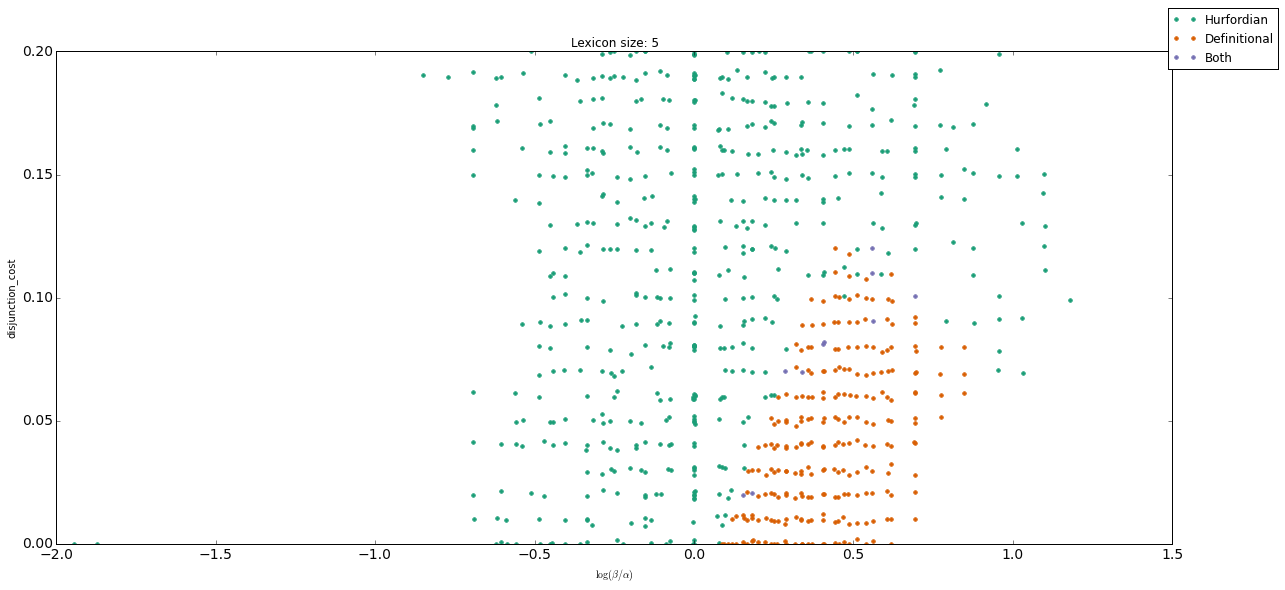
\includegraphics[width=1\textwidth]{fig/lex5-alpha-beta-gamma}
  \caption{Hurfordian and definitional contexts with a large
    lexicon (five atomic lexical items, four atomic states).} 
  \label{fig:char}
\end{figure}

The above illustrative examples begin to show that $\beta$'s
relationship to the parameter $\alpha$ and the cost of disjunction are
what steer the discourse participants to exclusivization or
identification. \Figref{fig:char} seeks to offer get a fuller picture
of these dynamics using our larger lexicon setting (five atomic
messages, four atomic states). The x-axis gives $\log(\beta/\alpha)$
for values of $\alpha$ and $\beta$ between $0$ and $14$ inclusive. The
log-scale helps bring out the underlying relationships, and it also
means that values above $0$ are where $\beta$ is bigger than
$\alpha$. The y-axis gives the cost of disjunction, ranging from $0$
to $0.2$. The dots are samples from this space of parameters, with
green marking strictly dominant Hurford stratgies, orange marking
strictly dominant definitional strategies, and purple marking cases
where both strategies are strictly dominant (which is possible because
we've reduced $\alpha$ and $\beta$ to a single measure in order to
visualize the space).

The picture that emerges from \figref{fig:char} is relatively clear:
definitional readings exist in a narrow space where $\beta > \alpha$
and disjunction costs are low. As we said above, this makes intuitive
sense: where costs are high, the disjunction has to be
justified. Letting the two terms overlap reduces the justification,
whereas exclusivizing provides justification with regard to
$\alpha$. In other words, the apparently undue prolixity of the
disjunction (the more general term would seem to suffice!) generates
an inference that we observe in the lexical inferences. However, this
needs to be qualified by the speaker's desire to communicate about the
lexicon. If $\beta$ is high, then it might be worth paying the
disjunction costs for the sake of teaching the listener about the
lexicon, even if this involves a huge penalty in terms of
informativity (since definitional readings convey only a single term's
worth of information).

From this perspective, it is clear why Hurfordian uses are more
robust. They arise in a much wider range of parameters settings, that
is contexts, because they can easily survive high disjunction costs
--- exclusivization ensure genuine communicative value. In contrast,
definitional readings exist mainly in the space of low disjunction and
high $\beta$ because the state information they convey is fully
encoded in the first disjunct, making the full disjunction an
inefficient way of conveying world information.

Focal points: \figref{fig:char-focal}.

\begin{figure}[tp]
  \centering
  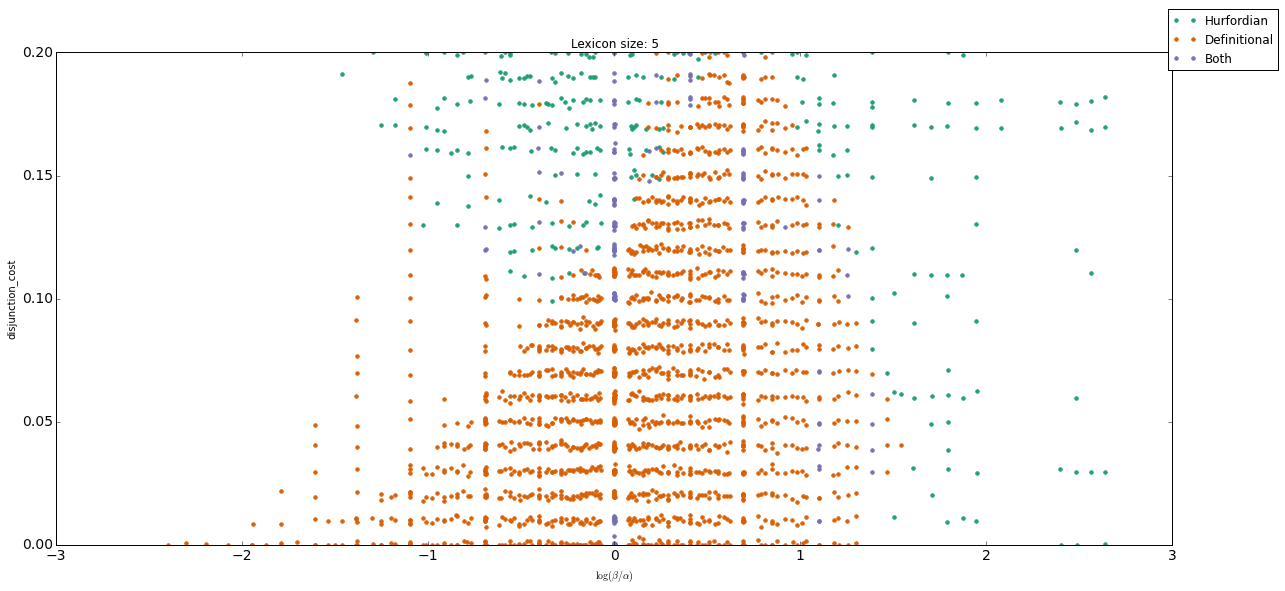
\includegraphics[width=1\textwidth]{fig/lex5-alpha-beta-gamma-X}
  \caption{A focal point unknown word. Hurfordian and definitional contexts with 
    lexicon (five atomic lexical items, four atomic states).} 
  \label{fig:char-focal}
\end{figure}


%%%%%%%%%%%%%%%%%%%%%%%%%%%%%%%%%%%%%%%%%%%%%%%%%%%%%%%%%%%%%%%%%%%%%%

\section{Conclusion}\label{sec:conclusion}

Importance of secondary information, lexical negotiations, variable
expertise.

Communicating in language about language. Maybe mention other areas
where we do those.

Broader perspective on recursive Bayesian models and their role in
semprag.

Potential to bring in social dimensions, pedagogical dimensions, ...

Perhaps notes about future behavioral experiments --- challenges of
running them, virtues of having the data, ability of our model to make
quantitative predictions given measured priors and costs.

%%%%%%%%%%%%%%%%%%%%%%%%%%%%%%%%%%%%%%%%%%%%%%%%%%%%%%%%%%%%%%%%%%%%%%

\bibliographystyle{apalike}
\bibliography{levy-potts-pragdisj-bib}

\end{document}


